% TODO:
%   - Adjust Jacobian of process noise w.r.t. process noise (add T_km1 terms).
\documentclass[ nobib, nofonts, notoc]{tufte-handout}
\usepackage{amro-common}
\usepackage{amro-tufte}
\makeatletter
% Remove paragraph indentation
\renewcommand{\@tufte@reset@par}{%
  \setlength{\RaggedRightParindent}{0.0pc}%
  \setlength{\JustifyingParindent}{0.0pc}%
  \setlength{\parindent}{0pc}%
  \setlength{\parskip}{\baselineskip}%
}
\@tufte@reset@par

% Paragraph indentation and separation for marginal text
\renewcommand{\@tufte@margin@par}{%
  \setlength{\RaggedRightParindent}{0.5pc}%
  \setlength{\JustifyingParindent}{0.5pc}%
  \setlength{\parindent}{0.5pc}%
  \setlength{\parskip}{0pt}%
}
\makeatother

% % Might prevent marginnotes from jumping to another page
% \def\mathnote#1{%
%   \tag*{\rlap{\hspace\marginparsep\smash{\parbox[t]{\marginparwidth}{%
%   \footnotesize#1}}}}
% }


% % This command is needed for building in linux
% \captionsetup{compatibility=false}

\newcommand{\lplus}{\overset{{\scriptscriptstyle\mathrm{L}}}{\oplus}}
\newcommand{\liplus}{\overset{{\scriptscriptstyle\mathrm{LI}}}{\oplus}}
\newcommand{\rplus}{\overset{{\scriptscriptstyle\mathrm{R}}}{\oplus}}
\newcommand{\riplus}{\overset{{\scriptscriptstyle\mathrm{RI}}}{\oplus}}
% Ominus
\newcommand{\lminus}{\overset{{\scriptscriptstyle\mathrm{L}}}{\ominus}}
\newcommand{\liminus}{\overset{{\scriptscriptstyle\mathrm{LI}}}{\ominus}}
\newcommand{\rminus}{\overset{{\scriptscriptstyle\mathrm{R}}}{\ominus}}
\newcommand{\riminus}{\overset{{\scriptscriptstyle\mathrm{RI}}}{\ominus}}



\title{Batch Estimation}
\author{Amro Al~Baali}

% Generates the index
\usepackage{makeidx}
\makeindex

\setcounter{tocdepth}{2}


\begin{document}
    % \frontmatter
    {
        \makeatletter
\begin{titlepage}
    \begin{fullwidth}    
        \begin{center}
            
            % \vspace*{cm}
                
            % % \includegraphics[width=0.3\textwidth]{figs/McGill_Wordmark.png}
            % \vspace{0.5cm}
            
            % \Huge
            % \textsc{McGill University}
            % \vspace{0.5cm}
            
            % \Huge
            % \textsc{DECAR Group}
            
            % \vspace{0.5cm}
            
            \LARGE
            \textsc{Notes}
            
            \vspace{5cm}
            
            \Huge
            % \thline
            \vspace{0.6em}
            \textbf{\@title}
            % \thline
            
            \vfill
            
            \Large
            {\@author}\\[10pt]
            % 26062940\\[10pt]
            % \textit{Supervisor:}\\
            % {Prof.} {James Richard Forbes}\\[10pt]
            

            % \large
            % Department of Mechanical Engineering, McGill University\\
            % 817 Sherbrooke Street West, Montreal, QC, H3A 0C3\\[10pt]
            
            \today
            
        \end{center}    
    \end{fullwidth}
\end{titlepage}
        % \forceheader{Contents}
        \tableofcontents
        \clearpage
        % \thispagestyle{empty}
        % \addtocontents{toc}{\protect\thispagestyle{empty}}
    }
    % \mainmatter

    %%%%%%%%%%%%%%%%%%%%%%%%%%%%%%%%%%%%%%%%%%%%%%%%%%%%%%%%%%%%%%%%%%%%%%%%%%%%%%
    % Why this document?
    %%%%%%%%%%%%%%%%%%%%%%%%%%%%%%%%%%%%%%%%%%%%%%%%%%%%%%%%%%%%%%%%%%%%%%%%%%%%%%
    \section{Why this document?}
    This document will be used as a guide to batch estimation on design variables that live in Lie groups. It'll be assumed that the random variables follow a Gaussian distribution. Therefore, the state estimation problem boils down to some least squares problem.

    %%%%%%%%%%%%%%%%%%%%%%%%%%%%%%%%%%%%%%%%%%%%%%%%%%%%%%%%%%%%%%%%%%%%%%%%%%%%%%
    % Linear least squares
    %%%%%%%%%%%%%%%%%%%%%%%%%%%%%%%%%%%%%%%%%%%%%%%%%%%%%%%%%%%%%%%%%%%%%%%%%%%%%%
    \section{Linear least squares}
    Linear least squares is a special type of unconstrained optimization problem. It has the form
    \begin{align}
        \label{eq:optim problem linear least squares}
        \min_{\mbf{x}\in\rnums^{n}}
        &\f{1}{2}\left( \mbf{A} \mbf{x} - \mbf{b} \right)^{\trans}\left( \mbf{A}\mbf{x} - \mbf{b} \right).
    \end{align}
    \marginnote[-1cm]{The error function is really \emph{affince}, but that's how it is.}
    The objective function can be expanded to a quadratic form
    \begin{align}
        J(\mbf{x})
        &= \f{1}{2}\left( \mbf{A} \mbf{x} - \mbf{b} \right)^{\trans}\left( \mbf{A}\mbf{x} - \mbf{b} \right)\\
        &= \f{1}{2}\mbf{x}^{\trans}\mbf{A}^{\trans}\mbf{A}\mbf{x} - \mbf{b}^{\trans}\mbf{A}\mbf{x} + \f{1}{2}\mbf{b}^{\trans}\mbf{b}
    \end{align}
    which is a \emph{convex} function in $\mbf{x}$. Furthermore, the objective function is \emph{strongly} quadratic function if $\mbf{A}^{\trans}\mbf{A}$ is positive definite, which occurs if $\mbf{A}$ has full \emph{column rank}. \sidenote{This assumption is usually valid since it is common to have more measurements than the number of design variables.}

    If $\mbf{A}$ is full rank, then the optimization problem \eqref{eq:optim problem linear least squares} has a unique minimizer and is given by solving the linear system
    \begin{align}
        \label{eq:linear least squares normal equations}
        \mbf{A}^{\trans}\mbf{A}\mbf{x}^{\star} &= \mbf{A}^{\trans}\mbf{b}.
    \end{align}
    \marginnote[-1cm]{This equation is referred to as the \emph{normal equations} \cite{Dellaert_Factor_2017}.}

    There are efficient ways to solve \eqref{eq:linear least squares normal equations} than inverting $\mbf{A}^{\trans}\mbf{A}$. These include Cholesky and QR factorizations \cite{Golub_Matrix_2013,Dellaert_Factor_2017}.


    \subsection{Weighted least squares}
    Most often, weighted least squares optimization is used where the objective function is of the form
    \begin{align}
        \label{eq:weighted least squares: objective function using W}
        J(\mbf{x}) &= \f{1}{2}\left( \mbf{A}\mbf{x} - \mbf{b} \right)^{\trans}\mbf{W}\left(  \mbf{A}\mbf{x} - \mbf{b}\right),
    \end{align}
    where $\mbf{W}=\mbf{W}^{\trans}>0$ is a symmetric positive definite matrix.
    This form arises naturally in the maximum a posteriori (MAP) estimator over normally distributed measurements $\mbfrv{b}\sim\mc{N}\left( \mbf{b}, \mbs{\Sigma} \right)$, where the weight matrix is assigned $\mbf{W} = \mbs{\Sigma}\inv$ \cite{Barfoot_State_2017a}.

    However, since the weight matrix is positive definite, then the Cholesky decomposition can be used so that
    \begin{align}
        \mbf{L}^{\trans}\mbf{L} &= \mbf{W},
    \end{align}
    where $\mbf{L}$ is a lower triangular matrix. The $\mbf{L}$ matrix can then be inserted into the objective function \eqref{eq:weighted least squares: objective function using W} which results in
    \begin{align}
        J(\mbf{x})
        &= \f{1}{2}\left( \mbf{A}\mbf{x} - \mbf{b} \right)^{\trans}\mbf{W}\left(  \mbf{A}\mbf{x} - \mbf{b}\right)\\
        &=\f{1}{2}\left( \mbf{A}\mbf{x} - \mbf{b} \right)^{\trans}\mbf{L}^{\trans}\mbf{L}\left(  \mbf{A}\mbf{x} - \mbf{b}\right)\\
        &= \f{1}{2}\left( \mbf{L}\mbf{A}\mbf{x} - \mbf{L}\mbf{b} \right)^{\trans}\left( \mbf{L}\mbf{A}\mbf{x} - \mbf{L}\mbf{b}\right)\\
        &= \f{1}{2}\left( \mbftilde{A}\mbf{x} - \mbftilde{b} \right)^{\trans}\left( \mbftilde{A}\mbf{x} - \mbftilde{b}\right),
    \end{align}
    where
    \begin{align}
        \mbftilde{A} &= \mbf{L}\mbf{A},\\
        \mbftilde{b} &= \mbf{L}\mbf{b}.
    \end{align}
    The resulting form is a standard linear least squares problem.
    Therefore, without loss of generality, the least squares problem can be assumed to be of the form \eqref{eq:optim problem linear least squares}.

    %%%%%%%%%%%%%%%%%%%%%%%%%%%%%%%%%%%%%%%%%%%%%%%%%%%%%%%%%%%%%%%%%%%%%%%%%%%%%%
    % Euclidean nonlinear least squares
    %%%%%%%%%%%%%%%%%%%%%%%%%%%%%%%%%%%%%%%%%%%%%%%%%%%%%%%%%%%%%%%%%%%%%%%%%%%%%%
    \section{Euclidean nonlinear least squares}
    Nonlinear least squares optimization problem is given by
    \begin{align}
        \min_{\mbf{x}\in\mbf{R}^{n}} \f{1}{2}\mbf{e}(\mbf{x})^{\trans}\mbf{e}(\mbf{x}),
    \end{align}
    where $\mbf{e} : \rnums^{n} \to \rnums^{m}$ is some nonlinear \emph{error function}.

    One way to solve this optimization iteratively is by linearizing the error function $\mbf{e}(\mbf{x})$ at some operating point $\mbfbar{x}$. This results in the Gauss-Newton equation \cite{Barfoot_State_2017a,Dellaert_Factor_2017}.

    First, define the error on the optimizer. That is, let
    \begin{align}
        \label{eq:Euclidean NLS error}
        \mbf{x} &= \mbfbar{x} + \delta\mbf{x},
    \end{align}
    where $\mbfbar{x}$ is some operating point.\sidenote{The operating point will be updated at each iteration.} Plugging the error definition \eqref{eq:Euclidean NLS error} into the error function gives
    \begin{align}
        \mbf{e}(\mbf{x}) &= \mbf{e}(\mbfbar{x} +\delta\mbf{x})\\
        \label{eq:Euclidea NLS perturbed error}
        &\approx \mbf{e}(\mbfbar{x}) + \mbf{J}\delta\mbf{x},
    \end{align}
    where $\mbf{J}\in\rnums^{m\times n}$ is the Jacobian of the error function $\mbf{e}$ with respect to its design variables $\mbf{x}$.

    Plugging the perturbed error function \eqref{eq:Euclidea NLS perturbed error} into the objective function gives
    \begin{align}
        \tilde{J}(\delta\mbf{x}) &\coloneqq J(\mbfbar{x} + \delta\mbf{x})\\
        &= \f{1}{2}\mbf{e}(\mbfbar{x} + \delta\mbf{x})^{\trans}\mbf{e}(\mbfbar{x} + \delta\mbf{x})\\
        &\approx
        \f{1}{2}\left( \mbf{e}(\mbfbar{x}) + \mbf{J}\delta\mbf{x} \right)^{\trans} \left( \mbf{e}(\mbfbar{x}) + \mbf{J}\delta\mbf{x} \right)\\
        &= \f{1}{2}\delta\mbf{x}^{\trans}\mbf{J}^{\trans}\mbf{J}\delta\mbf{x} + \mbf{e}(\mbfbar{x})^{\trans}\mbf{J}\delta\mbf{x} + \f{1}{2}\mbf{e}(\mbfbar{x})^{\trans}\mbf{e}(\mbfbar{x})
    \end{align}
    which is a quadratic\sidenote{Quadratic in $\delta\mbf{x}$.} approximation of the objective function.

    If $\mbf{J}$ has full column rank, then $\tilde{J}(\delta\mbf{x})$ is a strongly quadratic function. The minimizer of $\tilde{J}(\delta\mbf{x})$ is then given by the solving the system of equations
    \begin{align}
        \mbf{J}^{\trans}\mbf{J}\delta\mbf{x}^{\star} &= -\mbf{J}^{\trans}\mbf{e}(\mbfbar{x}).
    \end{align}
    Again, this system of equations can be solved efficiently using Cholesky and QR factorizations.

    Finally, using the error definition \eqref{eq:Euclidea NLS perturbed error}, the operating point can be updated using
    \begin{align}
        \mbfbar{x}^{(j+1)} &= \mbfbar{x}^{(j)} + \delta\mbf{x}^{\star},
    \end{align}
    where the superscript $(j)$ is added to denote the Gauss-Newton iteration.

    Gauss-Newton may perform poorly if the residual is large \cite{Nocedal_Numerical_2006,Fletcher_Practical_1987}, thus it's advisable to use line search methods when updating the operating point. That is, use
    \begin{align}
        \mbfbar{x}^{(j+1)} &= \mbfbar{x}^{(j)} + \alpha^{(j)}\delta\mbf{x}^{\star},
    \end{align}
    where $\alpha^{(j)}$ is a step-length computed using some heuristics like backtracking \cite{Nocedal_Numerical_2006}.

    Another popular method is Levenberg-Marquardt \cite{Dellaert_Factor_2017,Nocedal_Numerical_2006} which can be thought of as a damped version of Gauss-Newton.

    %%%%%%%%%%%%%%%%%%%%%%%%%%%%%%%%%%%%%%%%%%%%%%%%%%%%%%%%%%%%%%%%%%%%%%%%%%%%%%
    % Non-Euclidean nonlinear least squares
    %%%%%%%%%%%%%%%%%%%%%%%%%%%%%%%%%%%%%%%%%%%%%%%%%%%%%%%%%%%%%%%%%%%%%%%%%%%%%%
    \section{Non-Euclidean nonlinear least squares}
    If the design variables\sidenote{Elements of Lie groups will be denoted by upper case boldface letters.} $\mbf{X}$ are elements of non-Euclidean space, say elements of a Lie group $G$,\sidenote{For example, the Special Euclidean group of rotations $SO(3)$.} then the Euclidean addition operator `$+$' wouldn't necessarily work.
    This complicates things a little bit, and a more generalized approach must be taken.

    The optimization problem will first take the form
    \begin{align}
        \min_{\mbf{X}\in G} \f{1}{2}\mbf{e}(\mbf{X})^{\trans}\mbf{e}(\mbf{X}),
    \end{align}
    where $\mbf{e} : G \to \mbf{R}^{m}$.

    The optimization problem can still be solved using Gauss-Newton method.
    As discussed in the previous section, the Jacobian of the error function with respect to the design variable is needed to compute the search direction.
    But what does that look like when the design variable is an element of a Lie group?
    A generalized `addition' operator $\oplus$' is used.

    For example, let $\mbf{X}\in SO(3)$ be an element of the $SO(3)$ group.
    Then the element $\mbf{X}$ can be perturbed by the column matrix $\mbs{\xi}\in\rnums^{3}$ that lives in the Euclidean space isomorphic to the tangent space $\mf{so}(3)$.
    The left-invariant increment operator `$\liplus$' over $SO(3)$ is then defined as
    \begin{align}
        \mbf{X} \liplus \mbs{\xi} &\triangleq \mbf{X}\exp(-\mbs{\xi}\crossop),
    \end{align}
     $(\cdot)\crossop$ is the skew-symmetric cross-operator defined as \cite{Barfoot_State_2017a}
    \begin{align}
        \bbm
            \xi_{1}\\
            \xi_{2}\\
            \xi_{3}
        \ebm\crossop
        &\triangleq
        \bbm
            0 & -\xi_{3} & \xi_{2} \\
            \xi_{3} & 0 & -\xi_{1}\\
            -\xi_{2} & \xi_{1} & 0
        \ebm.
    \end{align}

    Using such notation, the error function $\mbf{e}$ can be perturbed with respect to the Lie \emph{algebra} element (i.e., the $\mbs{\xi}\in\rnums^{n}$ element).
    The error function can then be perturbed to be of the form
    \begin{align}
        \mbf{e}(\mbf{X})
        &= \mbf{e}(\mbfbar{X}\oplus \delta\mbs{\xi})\\
        % &\approx \mbf{e}(\mbfbar{X}) + \mbf{J}^{\mbf{e}}_{\mbs{\xi}}\delta\mbs{\xi},
        &\approx \mbf{e}(\mbfbar{X}) + \mbf{J}\delta\mbs{\xi},
    \end{align}
    where $\mbf{J}\in\rnums^{m\times n}$.
    Sola~\cite{Sola_micro_2019} provides a good explanation of Jacobians over Lie groups elements.
    An example will be provided in the following sections.

    Just as in the Euclidean case, the Jacobian can then be used to compute the search direction
    \begin{align}
        \mbf{J}^{\trans}\mbf{J}\delta\mbs{\xi}^{\star} &= -\mbf{J}^{\trans}\mbf{e}(\mbfbar{X}).
    \end{align}
    Finally, the design variable can be updated can be updated using
    \begin{align}
        \mbf{X}^{(j+1)} &= \mbf{X}^{(j)}\oplus \left( \alpha^{(j)}\delta\mbs{\xi}^{\star} \right),
    \end{align}
    where $\alpha^{(j)}$ is the step-length computed and $\oplus$ is the defined increment operation.\sidenote{The perturbations are left-, right-, left-invariant-, and right-invariant-perturbations \cite{Sola_micro_2019,Barrau_Invariant_2018}.}

    %%%%%%%%%%%%%%%%%%%%%%%%%%%%%%%%%%%%%%%%%%%%%%%%%%%%%%%%%%%%%%%%%%%%%%%%%%%%%%
    % SE(2) Example
    %%%%%%%%%%%%%%%%%%%%%%%%%%%%%%%%%%%%%%%%%%%%%%%%%%%%%%%%%%%%%%%%%%%%%%%%%%%%%%
    \section[Example on the planar Special Euclidean group]{Example on $SE(2)$}
    \begin{marginfigure}%
        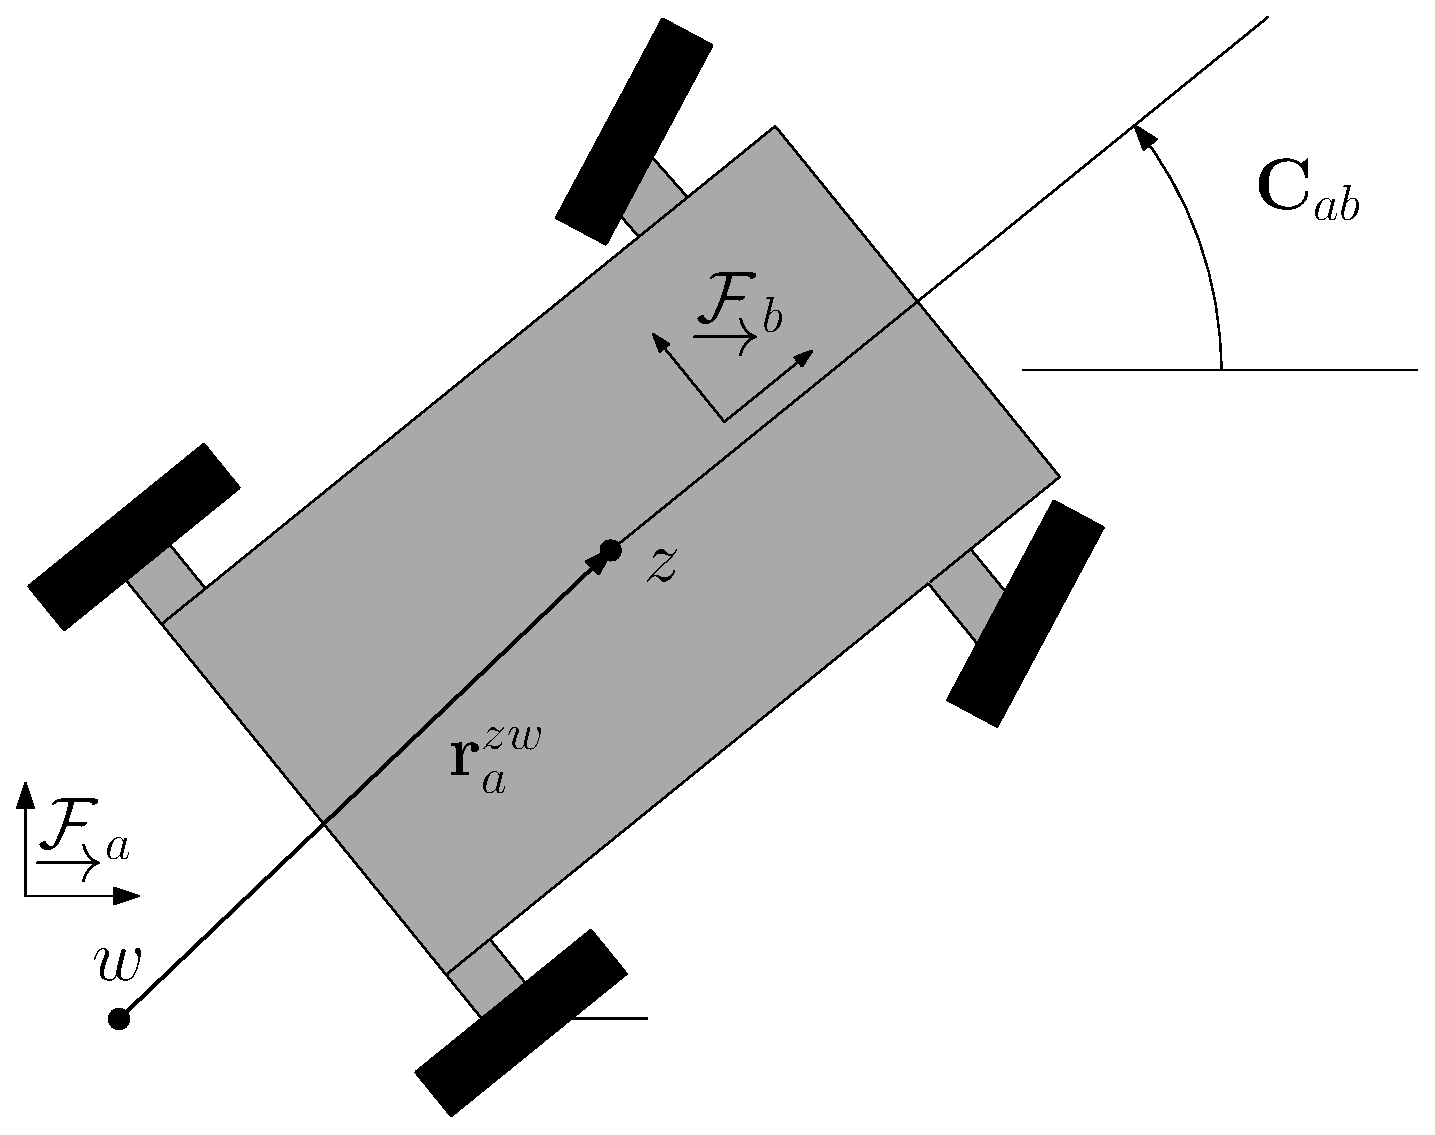
\includegraphics[width=\linewidth]{figs/Graphics/car_body.eps}
        \caption{Robot with point $z$ relative to point $w$. The body frame $\rframe[b]$ is attached to the robot, and reference frame $\rframe[a]$ is the reference frame.}
        \label{fig:car body}
    \end{marginfigure}
    %
    Consider a robot moving on a plan like the one displayed in \figref{fig:car body}.
    Let $z_{k}$ be a \emph{point} on attached to the robot and $w$ be a reference \emph{point}.
    Furthermore, let $\rframe[b_{k}]$ be the robot reference frame (at time $k$), and $\rframe[a]$ be the reference frame (e.g., some inertial frame).
    The robot can then be described by the \emph{pose}
    \begin{align}
        \pose[z_{k}w][ab_{k}] &=
        \bbm
            \dcm[ab_{k}] & \disp[z_{k}w][a] \\
            \mbf{0} & 1
        \ebm \in SE(2),
    \end{align}
    where $\dcm[ab_{k}]\in SO(2)$ and $\disp[z_{k}w][a]\in\rnums^{2}$.
    For simplicity and visual clarity, notation
    \begin{align}
        \mbf{X}_{k} \coloneqq \pose[z_{k}w][ab_{k}]
    \end{align}
    will be used in this document.\footnote{The $\mbf{X}$ is usually reserved for `design variable' so the Lie group should hopefully be inferred from the context.}

    \subsection{Process model}
    The process model is given by \cite{Barfoot_State_2017a}
    \begin{align}
        \mbfdot{X}(t) &= \mbf{X}(t)\Exp( \mbf{u}(t))\Exp(\rv{\boldsymbol{{w}}}(t)),
    \end{align}
    where
    \begin{align}
        \mbf{u}(t)
        &=
        \bbm
            \omega^{ba}_{b}(t)\\
            \mbf{v}^{zw / a}_{a}(t)
        \ebm,
    \end{align}
    are the \emph{interoceptive} measurements, and
    \begin{align}
        \rv{\boldsymbol{{w}}}(t) \sim \mc{GP}\left( \mbf{0}, \boldsymbol{Q}\delta(t-t') \right),
    \end{align}
    is a zero-mean white-noise Gaussian Process (GP) with power spectral density $\boldsymbol{Q}$ \cite{Barfoot_State_2017a}.

    The discrete-time kinematics can be described by\sidenote{Checkout \cite{Barfoot_State_2017a} for a more complete derivation.}
    \begin{align}
        \mbf{X}_{k}
        &= \mbf{X}_{k-1}\Exp( T_{k-1} \mbf{u}_{k-1})\Exp(\mbfrv{w}_{k-1})\\
        &= \mbf{X}_{k-1}\mbs{\Xi}_{k-1}\mbfrv{W}_{k-1},
    \end{align}
    where $T_{k-1}$ is the sampling period,
    \begin{align}
        \mbs{\Xi}_{k-1}
        &= \Exp(T_{k-1}\mbf{u}_{k-1})\\
        &= \exp(T_{k-1}\mbf{u}_{k-1}\expand),\\
        \mbf{u}_{k-1}\expand
        &=
        \bbm
            \left( \omega^{b_{k-1}a}_{b_{k-1}} \right)\crossop & \mbf{v}^{z_{k-1}w / a}_{a}\\
            \mbf{0} & 0
        \ebm,
    \end{align}
    and
    \begin{align}
        \mbf{w}_{k-1} \sim\mc{N}\left( \mbf{0}, \mbf{Q}_{k-1} \right),
    \end{align}
    is the process-noise and $\mbf{Q}_{k-1}$ is the process-noise covariance matrix. \sidenote[][-3cm]{
        If Euler discretization is used to compute the process-noise covariance matrix $\mbf{Q}_{k-1}$, then a correction must be made. Specifically, the covariance matrix would be given by
        \begin{align}
            \mbf{Q}_{k-1} &= \f{T_{k-1}^{2}}{T_{k-1}}\boldsymbol{Q}\\
            &= T_{k-1}\boldsymbol{Q},
        \end{align}
        where the $1/T_{k-1}$ scale factor corrects for intensity of the noise.
    }

    %%%%%%%%%%%%%%%%%%%%%%%%%%%%%%%%%%%%%%%%%%%%%%%%%%%%%%%%%%%%%%%%%%%%%%%%%%%%%%
    % GPS measurement model
    %%%%%%%%%%%%%%%%%%%%%%%%%%%%%%%%%%%%%%%%%%%%%%%%%%%%%%%%%%%%%%%%%%%%%%%%%%%%%%
    \subsection{GPS measurement model}
    The GPS measurement model is given by
    \begin{align}
        \mbf{y}_{k} &= \disp[z_{k}w][a] + \mbfrv{n}_{k},
    \end{align}
    where
    \begin{align}
        \mbfrv{n}_{k}\sim\mc{N}\left( \mbf{0}, \mbf{R}_{k} \right),
    \end{align}
    is measurement noise.

    Another way to write the measurement function in terms of the Lie group element $\mbf{X}_{k}\in SE(2)$ is
    \begin{align}
        \bbm
            \mbf{y}_{k}\\
            1
        \ebm
        &=
        \bbm
        \disp[z_{k}w][a] + \mbfrv{n}_{k}\\
        1
        \ebm\\
        &=
        \bbm
            \dcm[ab_{k}] & \disp[z_{k}w][a] \\
            \mbf{0} & 1
        \ebm
        \bbm
            \mbf{0} \\ 1
        \ebm
        +
        \bbm
            \mbfrv{n}_{k}\\
            0
        \ebm\\
        \label{eq:meas. model GPS Lie group}
        &=
        \mbf{X}_{k}\mbf{b} + \bbm \mbfrv{n}_{k} \\ 0 \ebm,
    \end{align}
    where
    \begin{align}
      \mbf{b}
      &=
      \bbm 0 & 0 & 1 \ebm^{\trans}.
    \end{align}

    %%%%%%%%%%%%%%%%%%%%%%%%%%%%%%%%%%%%%%%%%%%%%%%%%%%%%%%%%%%%%%%%%%%%%%%%%%%%%%
    % Process model error functions and Jacobians
    %%%%%%%%%%%%%%%%%%%%%%%%%%%%%%%%%%%%%%%%%%%%%%%%%%%%%%%%%%%%%%%%%%%%%%%%%%%%%%
    \subsection{Process model error functions and Jacobians}
    The left-invariant error on the process model is given by
    \begin{align}
        \mbf{e}^{\mathrm{odom}}_{k}\left(
            \mbf{X}_{k-1},
            \mbf{X}_{k},
            \mbf{w}_{k-1}
        \right)
        &=
        \Log
        \left(
            \mbf{X}_{k}\inv
            \mbf{X}_{k-1}
            \mbs{\Xi}_{k-1}
            \Exp(\mbf{w}_{k-1})
        \right)\\
        &=
        \log
        \left(
            \mbf{X}_{k}\inv
            \mbf{X}_{k-1}
            \mbs{\Xi}_{k-1}
            \Exp(\mbf{w}_{k-1})
        \right)
            \contract.
    \end{align}
    The Jacobian of the error function with respect to the Lie algebra elements $\mbs{\xi}_{j}$ for $j=k - 1, k$ as well as with respect to the process noise can be computed by perturbing the error function.
    Specifically,
    \begin{fullwidth}
        \begin{align}
            \mbf{e}^{\mathrm{odom}}_{k}
              \left(
                  \mbf{X}_{k-1},
                  \mbf{X}_{k},
                  \delta\mbf{w}_{k-1}
              \right)
            &=
            \mbf{e}^{\mathrm{odom}}_{k}
              \left(
                \mbfbar{X}_{k-1}
                  \liplus
                  \mbs{\xi}_{k-1},
                \mbfbar{X}_{k}
                  \liplus
                  \mbs{\xi}_{k},
                \delta\mbf{w}_{k-1}
              \right) \\
            &=
            \Log\left( \Exp(\mbs{\xi}_{k})
              \mbfbar{X}_{k}\inv
              \mbfbar{X}_{k-1}
              \Exp(-\mbs{\xi}_{k-1})
              \mbs{\Xi}_{k-1}
              \Exp(\delta\mbf{w}_{k-1})
            \right)\\
            &=
            \Log\left(
              \Exp(\mbs{\xi}_{k})
              \mbfbar{X}_{k}\inv
              \mbfbar{X}_{k-1}
              \mbs{\Xi}_{k-1}
              \mbs{\Xi}_{k-1}\inv
              \Exp(-\mbs{\xi}_{k-1})
              \mbs{\Xi}_{k-1}
              \Exp(\delta\mbf{w}_{k-1})
            \right)\\
            &=
            \Log\left(
              \Exp(\mbs{\xi}_{k})
              \mbfbar{X}_{k}\inv
              \mbfbar{X}_{k-1}
              \mbs{\Xi}_{k-1}
              \Exp(-\Adj{\mbs{\Xi}_{k-1}\inv}
              \mbs{\xi}_{k-1})
              \Exp(\delta\mbf{w}_{k-1})
            \right)\\
            &=
            \Log
            \left(
              \Exp(\mbs{\xi}_{k})
              \Exp\left( \mbfbar{e}^{\mathrm{odom}}_{k}\right)
              \Exp(-\Adj{\mbs{\Xi}_{k-1}\inv}\mbs{\xi}_{k-1})
              \Exp(\delta\mbf{w}_{k-1})
            \right)\\
            &\approx
            \mbfbar{e}^{\mathrm{odom}}_{k} +
            \mbf{J}^{\ell}(\mbfbar{e}^{\mathrm{odom}}_{k})\inv
            \delta\mbs{\xi}_{k}
            -\mbf{J}^{r}(\mbfbar{e}^{\mathrm{odom}}_{k})\inv
            \Adj{\mbs{\Xi}_{k-1}\inv}
            \delta\mbs{\xi}_{k-1}
            \Exp(\delta\mbf{w}_{k-1})
            \nonumber \\
            &\mathrel{\phantom{=}} \negmedspace{}
            +
            \mbf{J}^{r}(\mbfbar{e}^{\mathrm{odom}}_{k})\inv
            \delta\mbf{w}_{k-1},
        \end{align}
        where
        \begin{align}
            \mbfbar{e}^{\mathrm{odom}}_{k}
            &\coloneqq
            \mbf{e}
                ^{\mathrm{odom}}
                _{k}
                \left(
                  \mbfbar{X}_{k-1},
                  \mbfbar{X}_{k},
                  \mbf{0}
                \right),
        \end{align}
        and $\mbf{J}^{\ell}(\cdot)$ and $\mbf{J}^{r}(\cdot)$ are the left- and right-Jacobians of the $SO(2)$ group, respectively \cite{Barfoot_State_2017a}.
    \end{fullwidth}

    The Jacobians of the odometry error with respect to the Lie algebra perturbations are then given by
    \begin{align}
        \mbf{J}
            ^{\mbf{e}
                ^{\mathrm{odom}}
                _{k}}
            _{\mbs{\xi}_{k-1}}
        &=
        -\mbf{J}^{r}(\mbfbar{e}^{\mathrm{odom}}_{k})\inv
        \Adj{\mbs{\Xi}_{k-1}\inv}
        , \\
        \mbf{J}
            ^{\mbf{e}
                ^{\mathrm{odom}}
                _{k}}
            _{\mbs{\xi}_{k}}
        &=
        \mbf{J}^{\ell}(\mbfbar{e}^{\mathrm{odom}}_{k})\inv,
    \end{align}
    and the with respect to the process noise\sidenote{Or any random variable.} is given by
    \begin{align}
        \mbf{J}
            ^{\mbf{e}
                ^{\mathrm{odom}}
                _{k}}
            _{\mbf{w}_{k-1}}
        % &\coloneqq
        % \mbf{L}_{k-1}
        % \\
        &=
        \mbf{J}^{r}(\mbfbar{e}^{\mathrm{odom}}_{k})\inv.
    \end{align}
    \marginnote[-1cm]{
        This Jacobian of the process model error function w.r.t. process noise is usually denoted by $\mbf{L}_{k-1}$.
    }

    The covariance on the error function can the be (approximately) given by
    \begin{align}
        \cov{
            \mbf{e}
              ^{\mathrm{odom}}
              _{k}
            \left(
              \mbf{X}_{k-1},
              \mbf{X}_{k},
              \mbfrv{w}_{k-1}
            \right)
        }
        &\approx
        \mbf{J}
            ^{\mbf{e}
                ^{\mathrm{odom}}
                _{k}}
            _{\mbf{w}_{k-1}}
        \mbf{Q}_{k-1}
        {
        \mbf{J}
            ^{\mbf{e}
                ^{\mathrm{odom}}
                _{k}}
            _{\mbf{w}_{k-1}}
        }^{\trans}.
    \end{align}

    To find the answer, let's perturb the error function with respect to the process noise.
    %%%%%%%%%%%%%%%%%%%%%%%%%%%%%%%%%%%%%%%%%%%%%%%%%%%%%%%%%%%%%%%%%%%%%%%%%%%%%%
    % GPS measurement model error functions and Jacobians
    %%%%%%%%%%%%%%%%%%%%%%%%%%%%%%%%%%%%%%%%%%%%%%%%%%%%%%%%%%%%%%%%%%%%%%%%%%%%%%
    \subsection{GPS measurement model error functions and Jacobians}
    Using the measurement model \eqref{eq:meas. model GPS Lie group}, the error function is given by
    \begin{align}
      \label{eq:error function GPS}
      \bbm
        \mbf{e}^{\mathrm{GPS}}_{k} \\
        0
      \ebm
      &=
      \bbm
        \mbf{y}_{k} \\
        1
      \ebm
      -
      \mbf{X}_{k}\mbf{b}.
    \end{align}
    Perturbing the above error function with respect to the state, using a left-invariant error/perturbation gives
    \begin{align}
      \mbftilde{e}^{\mathrm{GPS}}_{k}
      &=
      \bbm
        \mbf{e}^{\mathrm{GPS}}_{k} \\
        0
      \ebm
      \\
      &=
      \bbm
        \mbf{y}_{k} \\
        1
      \ebm
      -
      \left(
        \mbfbar{X}_{k}
        \liplus
        \mbs{\xi}_{k}
      \right)\mbf{b}
      \\
      &=
      \bbm
        \mbf{y}_{k} \\
        1
      \ebm
      -
      \mbfbar{X}_{k}
      \exp\left(-\mbs{\xi}_{k}^{\wedge}\right)
      \mbf{b}
      \\
      &\approx
      \bbm
        \mbf{y}_{k} \\
        1
      \ebm
      -
      \mbfbar{X}_{k}
      \left(\eye-\mbs{\xi}_{k}^{\wedge}\right)
      \mbf{b}
      \\
      &=
      \underbrace{
        \bbm
        \mbf{y}_{k} \\
        1
        \ebm
        -
        \mbfbar{X}_{k}
        \mbf{b}
      }_{
          \bar{\mbftilde{e}}^{\mathrm{GPS}}_{k}
      }
      +
      \mbfbar{X}_{k}
      \mbs{\xi}_{k}^{\wedge}
      \mbf{b}
      \\
      &=
      \bbm
        \mbfbar{e}^{\mathrm{GPS}}_{k}\\
        0
      \ebm
      +
      \mbfbar{X}_{k}
      \mbf{b}^{\odot}
      \mbs{\xi}_{k}
      \\
      &=
      \bbm
        \mbfbar{e}^{\mathrm{GPS}}_{k}\\
        0
      \ebm
      +
      \bbm
        \mbf{0} & \dcmbar[ab_{k}] \\
           0    & \mbf{0}
      \ebm
      \mbs{\xi}_{k}.
    \end{align}
    Which results in
    \begin{align}
      \mbf{e}^{\mathrm{GPS}}_{k}
      &=
      \mbfbar{e}^{\mathrm{GPS}}_{k}
      +
      \bbm
        \mbf{0} & \dcmbar[ab_{k}]
      \ebm
      \mbs{\xi}_{k}
    \end{align}
    Therefore, the Jacobian of the GPS measurement error function \eqref{eq:error function GPS} is
    \begin{align}
      \mbf{J}^{
          \mbf{e}^{\mathrm{GPS}}_{k}
       }_{\mbs{\xi}_{k}}
       &=
       \bbm
         \mbf{0} &
         \dcmbar[ab_{k}]
       \ebm,
    \end{align}
    where $\dcmbar[ab_{k}]$ is the DCM of the robot at time $k$ at the linearization (i.e., at a Gauss-Newton iteration) point.

    \clearpage
    % \backmatter
    \bibliography{references}
    % \bibliographystyle{plainnat}
    \bibliographystyle{IEEEtran}
\end{document}